\documentclass{article}

\def\fileversion{0.1}
\def\filedate{2017/09/05}

\title{The \textsf{limecv} document class\thanks{This document corresponds to \textsf{limecv}~\fileversion, dated \filedate.}}

\author{Olivier Pieters \\ \texttt{me (at) olivierpieters (dot) be}}

\usepackage{listings}
\usepackage{tikz}
\usepackage{hyperref}

\usepackage{cleveref}
\usepackage{xparse}

\lstset{%
  basicstyle=\footnotesize\ttfamily, % font style and size
  breakatwhitespace=false,
  breaklines=true,
  numbers=left,
  numberstyle=\tiny,
  numbersep=5pt
}

\NewDocumentCommand{\cvRequirement}{m}{\textbf{#1}}

\begin{document}

\maketitle

\section{Introduction}

This document class is designed to facilitate easy development of curriculum vit\ae\ (CV) with this particular design. Special elements have been designed of particular sections to ease quick creation. This document class was co-designed with a business card, which can be found on GitHub: \url{https://github.com/opieters/business-card}.

The design of this CV is split up in three parts, illustated by \cref{design}. Each of these parts that make up this CV template, will be detailed in the sections below.

\begin{figure}[!ht]
  \centering
  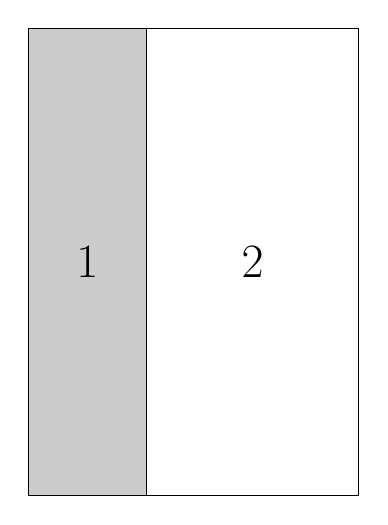
\begin{tikzpicture}
    \draw (0,0) rectangle ++(4.20,5.94);
    \draw[fill=black!20] (0,0) rectangle ++(1.5,5.94);
    \draw (0.75,2.97) node {\LARGE 1};
    \draw (2.85,2.97) node {\LARGE 2};
  \end{tikzpicture}%
  \hspace{2cm}%
  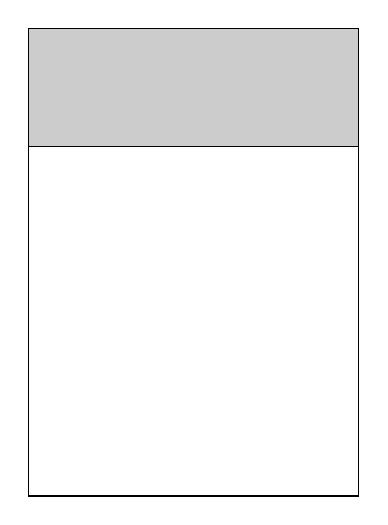
\begin{tikzpicture}
    \draw (0,0) rectangle ++(-4.20,-5.94);
    \draw[fill=black!20] (0,0) rectangle ++(-4.2,-1.5);
  \end{tikzpicture}
  \caption{Illustation of basic template. The left image depicts the actual CV: side bar to the left (1) with main content on the right (2). The right image depicts the cover letter design.}
  \label{design}
\end{figure}

\section{Requirements}

  Currently, it is advised to use the \cvRequirement{XeLaTeX} compiler. LaTeX will also work, but in that case icons are not available. In the subsequent, it will always be assumed that the XeLaTeX compiler is used (unless noted otherwise). 

  Any font can be used, though by default the \cvRequirement{Fira}\footnote{\url{https://github.com/mozilla/Fira}} font is used. This should be installed and accessable by the typesetting system. If another font is desired, it can be overwritten using the \lstinline|customfont| document class options and \lstinline|\cvMainFont| command. 

  \cvRequirement{FontAwesome}\footnote{\url{http://fontawesome.io}} is the icon font used. This font should also be available and cannot be replaced by another icon font. 

\section{General Macros and Document Class Options}

\section{Side Bar}

\section{Main Section}

\section{Cover Letter}

\section{Example}

  The source code of a typical CV document can be found below. \Cref{example-cv,example-cover-letter} depict the resulting PDF documents.

  \begin{figure}[!ht]
    \includegraphics[width=\textwidth,page=1]{mwe.pdf}
    \caption{Example CV (scaled).}
    \label{example-cv}
  \end{figure}

  \begin{figure}[!ht]
    \includegraphics[width=\textwidth,page=2]{mwe.pdf}
    \caption{Example cover letter (scaled).}
    \label{example-cover-letter}
  \end{figure}

  \lstinputlisting[language=tex]{mwe.tex}

\section{Source Code}

\lstinputlisting[language=tex]{limecv.cls}

\end{document}